\documentclass{article}%You can define the type of paper here.
%%Useful packages that I commonly use.
\usepackage[numbers]{natbib}%Bibliography package (help at http://merkel.zoneo.net/Latex/natbib.php).
\usepackage{url}%Package to highlight url.
\usepackage{times}%Sets font to be times.
\usepackage{alltt}%Allows the use of verbatim (good for printing out code).
\usepackage{graphicx}%Used to import images.
\usepackage{amsmath, amssymb, amscd, gensymb}%Contains the AMS expanded math symbols library.
%%For those who want smaller margins, you can use this:
\usepackage[top=1in, bottom=1in, left=1in, right=1in]{geometry}

\begin{document}

    %%Title
    \title{Simulation and Modeling\\Project III: Shallow Ice Approximations}
    \author{Clinton McKay}
    \maketitle

    %%Makes the paper use two collums
    \twocolumn

    %%Introduction-------------------------------------------------------------------------------------
    \section{Introduction}
    The focus of the project is to simulate ice flows and accumulation using the finite element method. 

    %%Method------------------------------------------------------------------------------------------
    \section{Method}
    The shallow ice approximation method simulates the motion of ice such that momentum is almost conserved by balancing the force of gravity and the resistance at the bed of the ice sheet. Our method will focus on converting the model presented by P. Huybrechts and T. Payne \cite{3}.

    \begin{align}
       0 &= \frac{\partial H}{\partial t} + \nabla D \nabla H - M\\
    \end{align}

    Simulating the system first required conversion into the weak form. 

    \begin{align}
        0 &= \int_\Omega\left[\frac{\partial H}{\partial t} * w + \cdot D \nabla H \cdot \nabla{w} - M * w\right]
    \end{align}

    The final step, make the formula implicit. 
 
    \begin{align}
        0 &= \int_\Omega\left[\frac{H^{n + 1} - H^n}{\partial t} * w + \cdot D \nabla H^{n + 1} \cdot \nabla{w} - M * w\right]
    \end{align}

    $H^n$ represents the elevation of the ice at step $n$. $D$ represents the approximation for the discharge which is a function that takes in $H^n$. 

    \begin{align}
        D(H) = \frac{2A(\rho g)^{n + 2}}{n + 2}  H^{n + 2}  \left[ \nabla H \cdot \nabla H\right]^{(n - 1)/2}
    \end{align}
    
    Where $A, \rho, g,$ and $n$ are a set of constants \cite{3}. 

    $M$ represents the accumulation rate of ice on the glacier. Given the scope of this project $M$ was only treated as either a constant and a value that was dependent it position in the system.  

    \begin{align}
        M &= min\{ 0.5, s(R_{el} - d\} \\
        d &= \sqrt{(x - x_{summet})^2 + (y - y_{summet})^2}
    \end{align}

    Such that $R_{el}, x_summet,$ and $y_summet$ represent the distance from which the mass balance switches from positive to negative, the $x$ center, and $y$ center of the system respectively. 

    %%Verification------------------------------------------------------------------------------------
    \section{Verification of Program}

    The model was simulated using FEniCS a project that provides tools for scientific computing using the finite element method. The project consists of two main files, {\it ShallowIce-VariablePrecip.py} and {\it ShallowIce-ConstantPrecip.py}. The first script contains code that simulates the shallow ice and assumes that $M = 0.3$. While the second script assumes that $M$ varies based on the position within the system and uses the formula (6) to model the accumulation rates.  

    %%Data--------------------------------------------------------------------------------------------
    \section{Data}
    Results after running the simulation with $M = 0.3$. 

    \begin{figure}[ht!]
        \centering
        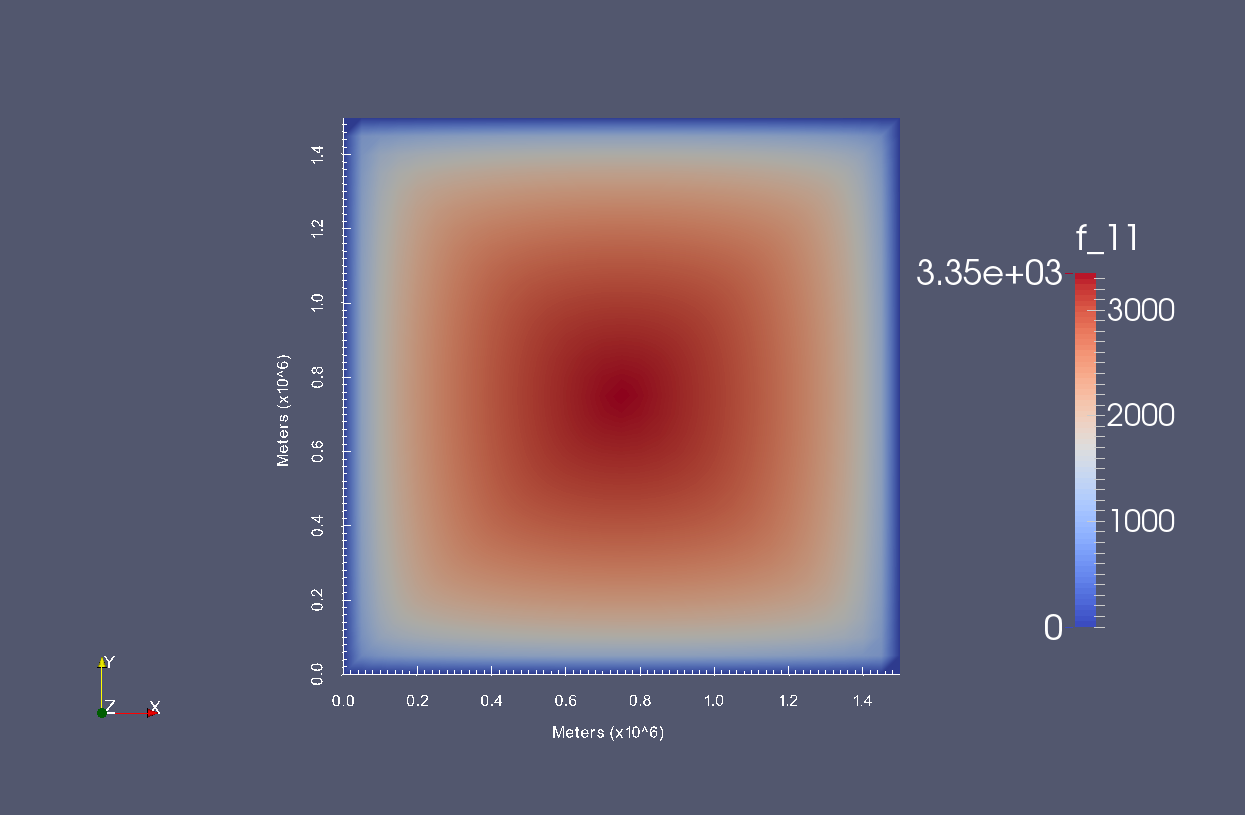
\includegraphics[width=3in]{../img/constant-accumulation.png} 
        \caption{ Results after running the simulation for $100,000$ years at a $1,000$ year time steps with $M = 0.3$ }
        \label{constant}
    \end{figure}

    \begin{figure}[ht!]
        \centering
        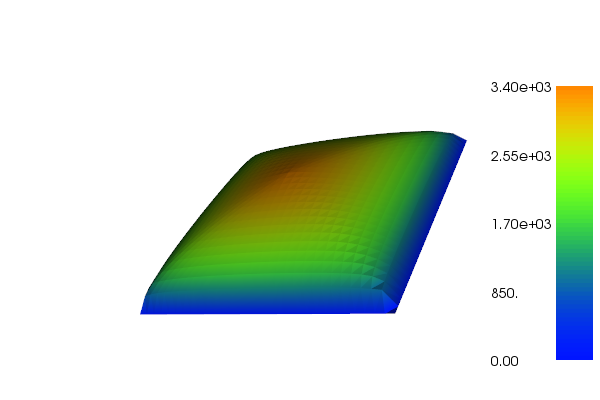
\includegraphics[width=3in]{../img/constant.png} 
        \caption{ 3-D view of figure \ref{constant} }
        \label{constant3d}
    \end{figure}

    Results after using dynamic accumulation rates. 

    \begin{figure}[h!]
        \centering
        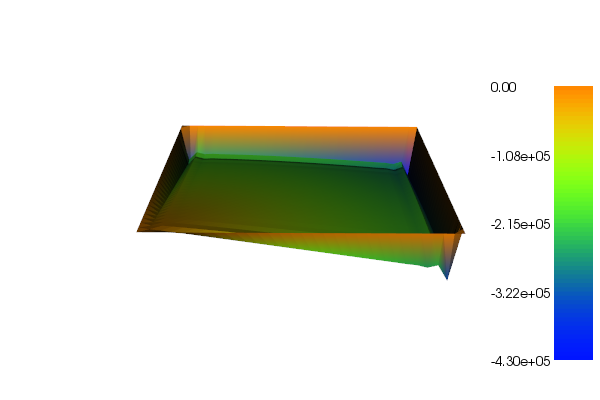
\includegraphics[width=3in]{../img/variable.png} 
        \caption{ Results after running the simulation for $100,000$ years at a $1,000$ year time steps. The simulation failed after the first time step.}
        \label{constant}
    \end{figure}

    %%Analysis---------------------------------------------------------------------------
    \newpage
    \section{Analysis}

    The first simulation produced a solution similar to the one shown on the project wiki. The highest point on the ice sheet was about 3.4 km in elevation. Near the edges the elevation tapered off to zero km. 

    The second simulation with the variable variable accumulation rates produced some rather interesting results. The edges of the sheet produced negative elevations at several thousand kilometers in depth. 
    
    %%Interpretation---------------------------------------------------------------------
    \section{Interpretation}

    Given the results of the first simulation, the model was properly implemented in FEniCS. As for the simulation that used the position dependent $M$ values. The simulation would fail at the first time step with FEniCS complaining that the model did not converge. The most likely candidates for the cause of the failure was the incorrect implementation of the formula or I didn't use it properly in FEniCS the weak form implementation.


    %%Critique---------------------------------------------------------------------------
    \section{Critique} 
    The introduction to the finite element method and FEniCS at the same time made the project difficult. Primarily because learning how to use FEniCS detracted from my focus on the finite element method. It would of been easier if we learned about it at the beginning of the semester.  

    %%Bibliography-----------------------------------------------------------------------
    \begin{thebibliography}{1}
        \bibitem{3} P. Huybrechts and T. Payne, The EISMINT benchmarks for testing ice-sheet models
        \bibitem{2} \url{http://wiki.cs.umt.edu/classes/cs477/index.php/The_Shallow_Ice_Approximation}
    \end{thebibliography} 

\end{document}
